

\tikzset{every picture/.style={line width=0.75pt}} %set default line width to 0.75pt        

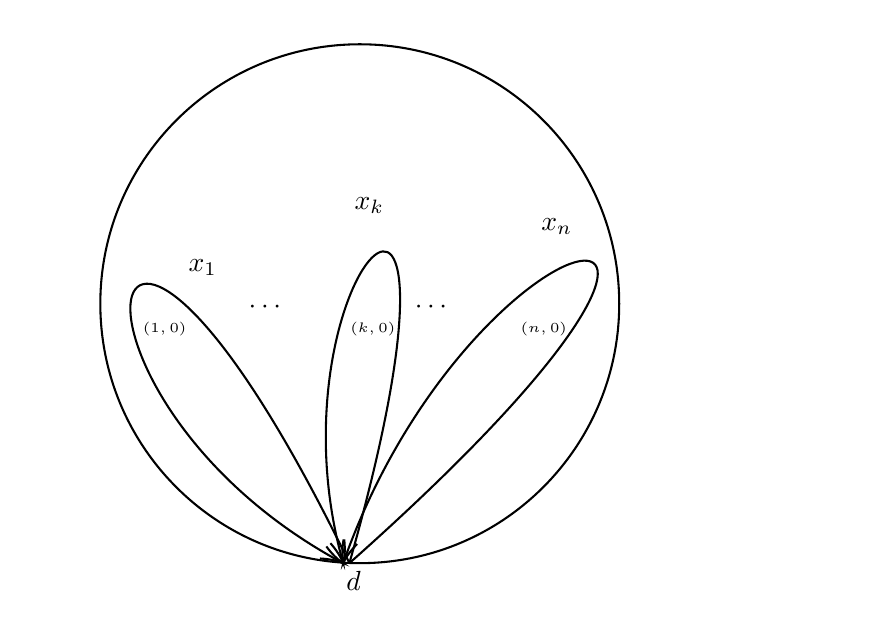
\begin{tikzpicture}[x=0.75pt,y=0.75pt,yscale=-1,xscale=1]
%uncomment if require: \path (0,877); %set diagram left start at 0, and has height of 877

%Shape: Circle [id:dp37495404303702484] 
\draw   (110,145) .. controls (110,75.96) and (165.96,20) .. (235,20) .. controls (304.04,20) and (360,75.96) .. (360,145) .. controls (360,214.04) and (304.04,270) .. (235,270) .. controls (165.96,270) and (110,214.04) .. (110,145) -- cycle ;
%Curve Lines [id:da24230856466474449] 
\draw    (230,270) .. controls (105,12.5) and (75.5,189) .. (227,270) ;
\draw [shift={(227,270)}, rotate = 208.13] [color={rgb, 255:red, 0; green, 0; blue, 0 }  ][line width=0.75]    (10.93,-3.29) .. controls (6.95,-1.4) and (3.31,-0.3) .. (0,0) .. controls (3.31,0.3) and (6.95,1.4) .. (10.93,3.29)   ;
%Curve Lines [id:da3024014633497575] 
\draw    (230,270) .. controls (302,16) and (188,131.5) .. (227,270) ;
\draw [shift={(227,270)}, rotate = 254.27] [color={rgb, 255:red, 0; green, 0; blue, 0 }  ][line width=0.75]    (10.93,-3.29) .. controls (6.95,-1.4) and (3.31,-0.3) .. (0,0) .. controls (3.31,0.3) and (6.95,1.4) .. (10.93,3.29)   ;
%Curve Lines [id:da03668887248571462] 
\draw    (230,270) .. controls (467,59.5) and (289.5,92.5) .. (227,270) ;
\draw [shift={(227,270)}, rotate = 289.4] [color={rgb, 255:red, 0; green, 0; blue, 0 }  ][line width=0.75]    (10.93,-3.29) .. controls (6.95,-1.4) and (3.31,-0.3) .. (0,0) .. controls (3.31,0.3) and (6.95,1.4) .. (10.93,3.29)   ;

% Text Node
\draw (129,152.4) node [anchor=north west][inner sep=0.75pt]  [font=\tiny]  {$( 1,0)$};
% Text Node
\draw (311,152.4) node [anchor=north west][inner sep=0.75pt]  [font=\tiny]  {$( n,0)$};
% Text Node
\draw (229,152.4) node [anchor=north west][inner sep=0.75pt]  [font=\tiny]  {$( k,0)$};
% Text Node
\draw (227,272.4) node [anchor=north west][inner sep=0.75pt]    {$d$};
% Text Node
\draw (180,142.4) node [anchor=north west][inner sep=0.75pt]    {$\cdots $};
% Text Node
\draw (260,142.4) node [anchor=north west][inner sep=0.75pt]    {$\cdots $};
% Text Node
\draw (151,122.4) node [anchor=north west][inner sep=0.75pt]    {$x_{1}$};
% Text Node
\draw (231,92.4) node [anchor=north west][inner sep=0.75pt]    {$x_{k}$};
% Text Node
\draw (321,102.4) node [anchor=north west][inner sep=0.75pt]    {$x_{n}$};


\end{tikzpicture}